\chapter{The VServer Control Daemon}
\label{ch:intro:vcd}


\section{Abstract}
\label{sec:intro:vcd:abstract}

In order to ease management of Virtual Private Servers a central instance is
needed to provide an open and well-known \emph{Application Programming
Interface (API)} not only for local, but especially for remote usage and
execution.  The \emph{VServer Control Daemon (VCD)} is a daemon running
in the host context and provides the aforementioned API using \emph{XML-RPC}, a
simple protocol for \emph{Remote Procedure Calls (RPC)} using the XML Markup
Language.


\section{Rationale}
\label{sec:intro:vcd:rationale}

The current user-space implementation of the Linux-VServer kernel API suffers a
mechanism to call any of the management commands regardless of the language or
location of the caller. Such callers include non-C lanuages like Python, PHP or
Ruby, remote GUIs for KDE, Gnome or even Windows as well as web control panels
for service providers.

Therefore the VServer Control Daemon defines an API accessible by any caller
capable of both the HTTP and the XMLRPC protocol -- two open standards
implemented in most common languages.


\section{Architecture}
\label{sec:intro:vcd:architecture}

The complete VServer Control Daemon package consists of four independent
modules:

\begin{labeling}[~~]{\labelingfont{vwrappers}}
	\labelingitem{libvserver} The libvserver module contains a library that implements
		the Linux-VServer system call in the C language. It provides a convenient
		way to execute Linux-VServer commands in other programs or libraries.
		Additionally basic low-level command-line tools are provided to work with
		these commands.

	\labelingitem{vcd} The VServer Control Daemon module uses -- among other
		libraries -- libvserver to implement the core of the package. This modules
		includes the configuration storage backend, the XML-RPC server,
		command-line clients and the kernel user-space helper.

	\labelingitem{vwrappers} The vwrappers module contains a lot of wrappers for
		coreutils/util-linux/procps and other system packages. This provides a
		convenient way to execute commands inside virtual private servers.
		Additionally, some utilities for the extended filesystem attributes are
		provided enhancing the versions in libvserver with recursion and various
		other options.

	\labelingitem{vstatd} The VServer Statistics Daemon module contains a \emph{very}
		small daemon that keeps track of resource utilization of virtual private
		servers. For statistical analysis all collected data is stored in a
		round-robin database (RRD), the industry standard data logging and graphing
		application.
\end{labeling}

A detailed descriptions of these modules can be found in the next sections.
However, the reader may skip to part~\ref{pt:install} on
page~\pageref{pt:install} for the installation guide and jump back here
occasionally once a more detailed module explanation is needed.


\section{Linux-VServer system call library}
\label{sec:intro:vcd:libvserver}

The Linux-VServer project provides an interface to the various virtualization
and configuration commands that have been added to the kernel. This interface
between the operating system and the user programs or libraries is known as
\emph{system call}.

For a long time the Linux-VServer project used a few different system calls to
accomplish different aspects of virtualization and configuration. However, the
number of commands grew rapidly and a few system calls were simply not enough to
handle every aspect of virtualization. Therefore, the Linux-VServer system call
now uses a system call multiplexer based on a command identifier, which has
similar semantics like the \texttt{ioctl} system call.

The Linux kernel maintainers have reserved a system call number for the
Linux-VServer project on most architectures meanwhile  and while the opinion on
system call multiplexing might differ from developer to developer, it was
generally considered a good decision not to have more than one syscall \ldots

The advantage of different system calls would be simpler handling on different
architectures. However, this has not been a problem so far, as the data passed
to and from the kernel has strong typed fields conforming to the C99 types.

The Linux-VServer system call requires three arguments regardless of what the
actual command is:

\begin{quote}
\texttt{sys\_vserver(uint32\_t cmd, uint32\_t id, void \_\_user *data);}
\end{quote}

\begin{labeling}{\labelingfont{data}}
\labelingitem{cmd}  a command number
\labelingitem{id}   an identifier
\labelingitem{data} a user-space data-structure of yet unknown size
\end{labeling}

To allow for some structure for debugging purposes and some kind of command
versioning, the command number is split into three parts: the lower 12 bit
contain a version number, then 4 bits are reserved, the upper 16 bits are
divided into 8 bit for the command number and 6 bit for category number, again
reserving 2 bits for the future.

In theory, there are 64 categories with up to 256 commands in each category,
allowing for 4096 revisions of each command, which is far more than will ever be
required.

The following categories and commands are defined in the Linux-VServer 2.2.0
release:

\begin{center}
\small
\begin{verbatim}
       |VERSION|CREATE |MODIFY |MIGRATE|CONTROL|EXPERIM| |SPECIAL|SPECIAL|
       |STATS  |DESTROY|ALTER  |CHANGE |LIMIT  |TEST   | |       |       |
       |INFO   |SETUP  |       |MOVE   |       |       | |       |       |
-------+-------+-------+-------+-------+-------+-------+ +-------+-------+
SYSTEM |VERSION|VSETUP |VHOST  |       |       |       | |DEVICES|       |
HOST   |     00|     01|     02|     03|     04|     05| |     06|     07|
-------+-------+-------+-------+-------+-------+-------+ +-------+-------+
CPU    |       |VPROC  |PROCALT|PROCMIG|PROCTRL|       | |SCHED. |       |
PROCESS|     08|     09|     10|     11|     12|     13| |     14|     15|
-------+-------+-------+-------+-------+-------+-------+ +-------+-------+
MEMORY |       |       |       |       |       |       | |SWAP   |       |
       |     16|     17|     18|     19|     20|     21| |     22|     23|
-------+-------+-------+-------+-------+-------+-------+ +-------+-------+
NETWORK|       |VNET   |NETALT |NETMIG |NETCTL |       | |SERIAL |       |
       |     24|     25|     26|     27|     28|     29| |     30|     31|
-------+-------+-------+-------+-------+-------+-------+ +-------+-------+
DISK   |       |       |       |       |DLIMIT |       | |INODE  |       |
VFS    |     32|     33|     34|     35|     36|     37| |     38|     39|
-------+-------+-------+-------+-------+-------+-------+ +-------+-------+
OTHER  |VSTAT  |       |       |       |       |       | |VINFO  |       |
       |     40|     41|     42|     43|     44|     45| |     46|     47|
=======+=======+=======+=======+=======+=======+=======+ +=======+=======+
SPECIAL|EVENT  |       |       |       |FLAGS  |       | |       |       |
       |     48|     49|     50|     51|     52|     53| |     54|     55|
-------+-------+-------+-------+-------+-------+-------+ +-------+-------+
SPECIAL|DEBUG  |       |       |       |RLIMIT |SYSCALL| |       |COMPAT |
       |     56|     57|     58|     59|     60|TEST 61| |     62|     63|
-------+-------+-------+-------+-------+-------+-------+ +-------+-------+
\end{verbatim}
\end{center}

While a single system call is advantageous from the kernel point of view,
user programs and libraries tend to have a single function per command, although
this is not always the case for multiplexed system calls, as can be seen with
\texttt{ioctl}. Nevertheless, the libvserver module implements a function for
each command the Linux-VServer multiplexer knows about.

For this purpose, the library uses acustom  syscall implementation written by
Herbert Pötzl in inline assembler rather than using the syscall macros provided
by \texttt{libc} to make the library as self-contained as possible.

The complete documentation of the libvserver API can be found on the projects
website~\cite{libvserver-doc} and is not discussed in further detail here.


\section{VServer Control Daemon}
\label{sec:intro:vcd:vcd}

The Vserver Control Daemon is the core of the the package and implements all
aspects of virtual server management using libvserver to issue Linux-VServer
system calls, xmlrpc-c to implement the XML-RPC protocol and SQLite3 for
data storage. Figure~\ref{fig:vcd-overview} illustrates the basic relationship
between libraries, methods and clients.

\begin{figure}[hbt]
	\center
	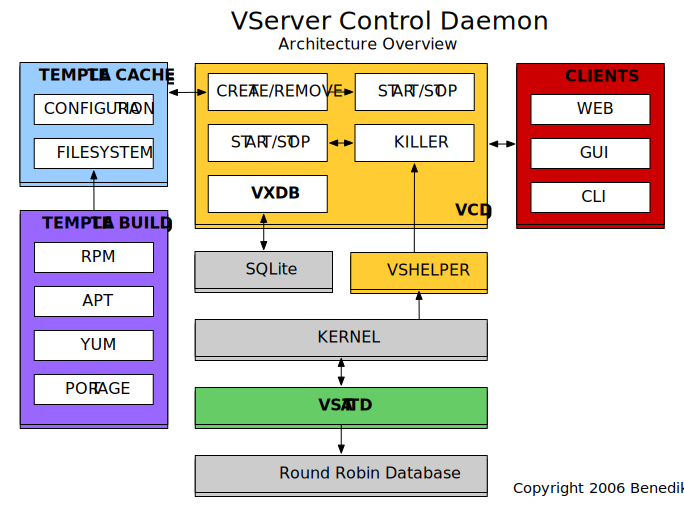
\includegraphics[scale=0.4]{intro/vcd}
	\caption{VServer Control Daemon Architecture Overview}
	\label{fig:vcd-overview}
\end{figure}


\subsection{Configuration Database - VXDB}

The configuration database (\emph{VXDB}) stores all virtual private server
related configuration data like disk limits, CPU scheduler buckets, or network
adresses. Furthermore the daemon stores information about its users and access
control as well as owner information in the database. For convenience and size
reasons the database is implemented using \emph{SQLite3}.

SQLite3 is a small C library that implements a self-contained, embeddable,
zero-configuration SQL database engine. The decision for using SQLite as
database backend is based on the following key-features of SQLite:

\begin{itemize}
	\item Transactions are atomic, consistent, isolated, and durable even
		after system crashes and power failures
	\item Zero-configuration - no setup or administration needed
	\item A complete database is stored in a single disk file
	\item Database files can be freely shared between machines with different
		byte orders
	\item Small code footprint: less than 250KB
	\item Faster than popular client/server database engines for most common
		operations
	\item Simple, easy to use API
	\item Self-contained: no external dependencies
\end{itemize}

\subsection{The XML-RPC Server}

The \emph{XML-RPC Server} is the core of the VServer Control Daemon and
implements the XML-RPC standard for Remote Procedure Calls (RPC). XMLRPC is a
specification and a set of implementations that allow software running on
disparate operating systems, running in different environments to make
procedure calls over the Wide Area Network (Internet) or Local Area Network
(Intranet).


\subsubsection{The XML-RPC Protocol}

XML-RPC is a wire protocol that describes an XML serialization format that
clients and servers use to pass remote procedure calls to each other. There are
two features that make this protocol worth knowing. The first is that the
details of parsing the XML are hidden from the user. The second is that clients
and servers don't need to be written in the same language.

XML-RPC is designed to be as simple as possible, while allowing complex data
structures to be transmitted, processed and returned. Figure~\ref{fig:xmlrpc}
illustrates the serialzation/deserialization in an XML-RPC session.

\begin{figure}[hbt]
	\center
	\includegraphics[scale=0.5]{intro/xmlrpc}
	\caption{XMLRPC data flow}
	\label{fig:xmlrpc}
\end{figure}

Here are some examples of remote procedure call (RPC) style communications:

\begin{itemize}
	\item There is a server that can measure atmospheric temperature. A client
		anywhere in the world can ask the server at any time what the
		temperature is. The ``what temperature is it?'' request and the
		``the temperature is...'' response constitute an RPC transaction.
	\item There is a server that can turn a light on or off. A client can tell
		the server to turn the light on. A request to turn the light on and
		the acknowledgement that the light has been turned on constitute an
		RPC transaction.
	\item There is a server that knows the phone numbers of a million people.
		A client can supply a name and get back the phone number of the named
		person.
\end{itemize}

Here are some kinds of communication that are not RPC:

\begin{itemize}
	\item A long-lived connection such as an SSH login session.
	\item A high volume transfer such as an FTP download.
	\item A one-way transmission such as a UDP packet.
	\item A dialogue such as an SMTP (mail) transaction.
\end{itemize}

Based on XML nearly any application can be enabled to call methods defined by
the XML-RPC Server. Additionally, the fact that XML is written in plain-text
and also easily parsable by humans allows easy tracing and debugging of XML-RPC
sessions in case of failure or other strange behaviour.

On startup, the server defines a global registry of methods accessible by its
clients. In order to allow structure for the amount of methods currently
defined, all methods are devided in logical units -- also known as namespaces --
and prefixed with the namespace and a dot, like \verb,vx.start, or
\verb,helper.shutdown, for the start and shutdown methods of the vx and helper
namespace, respectively.

Refer to part~\ref{pt:rpcref} on page~\pageref{pt:rpcref} for a detailed
description of the XML-RPC protocol and the request and response format used
for defined methods.

\subsubsection{Authentication}

Authentication in the VServer Control Daemon is based on the cryptographic hash
function \emph{WHIRLPOOL}. WHIRLPOOL is a cryptographic hash function designed
by Vincent Rijmen and Paulo S. L. M. Barreto. The hash has been recommended by
the NESSIE project. It has also been adopted by the International Organization
for Standardization (ISO) and the International Electrotechnical Commission
(IEC) as part of the joint ISO/IEC 10118-3 international standard.

WHIRLPOOL is a hash designed after the Square block cipher. WHIRLPOOL is a
Miyaguchi-Preneel construction based on a substantially modified Advanced
Encryption Standard (AES).  Given a message less than 2256 bits in length, it
returns a 512-bit message digest.

For security reasons the clear-text password is never stored in VXDB. The
client will send the password as plain-text -- the server then creates a
WHIRLPOOL hash using the submitted password and compares its result with the
hash stored in VXDB. It is also possible to create the hash on the client side,
prefix the result with \verb,WHIRLPOOLENC//, and send the result to the server
for authentication. The server then compares the hash after the prefix.

Note that an attacker can still authenticate against the server with the hash
only, he just cannot retreive the original password again. Therefore, the server
should \emph{never} listen on an untrusted network if no other security measures
have been setup, like an SSL or VPN tunnel.


\subsubsection{Access Restrictions}

For a fine-grained access control the server implements its own set of
capabilities.  A capability is a lot like a drivers license. As an example,
consider your car license. It allows you to drive a certain set of
vehicles (it designates a particular object set, in our case XML-PRC methods),
and anyone holding a car license is allowed to drive the same set of objects
(cars).

Refer to part~\ref{pt:rpcref} on page~\pageref{pt:rpcref} for a detailed
description of available access restrictions and their usage in defined methods.

\subsubsection{Owner Checks}

To ensure the distinction between your car and your neighbours Lamborghini
another access control system has to be implemented. Therefore the server also
implements owner checks for most of its methods. This results in an extension to
the capability model explained above. The server implements another object set
based on the ownership information stored in the database. Instead of allowing
everyone holding a certain capability to operate on all virtual servers, only
the intersection of both object sets is permitted for operation.

Still, this model has a noticable flaw: Imagine a company has two hundred cars
and the top management should have access to all cars. Adding all members
of the management to the owner list of every single car can become a pain in
the ass very quickly. Therefore the user database in VXDB implements an
additional configuration option~--~the adminstrator flag. Using this flag all
owner checks are passed without even consulting the owner lists in the database.


\subsection{XML-RPC Clients}

The \emph{XML-RPC Clients} provided in the VServer Control Daemon module
provide facilities to connect and execute methods on remote servers. Several
clients exist for different purpose, in most cases they are aligned with the
method namespaces mentioned above.

It is important to know that the connection between server and client is not
persistent, i.e. you send one request, get one answer, and the connection will
be closed afterwards. This also implies the necesity of passing authentication
information with every method call. After the request has been received and
processed the method returns a fault notification in case of any error or a
method specific return value.

Refer to part~\ref{pt:rpcref} on page~\pageref{pt:rpcref} for a detailed
description of the XML-RPC protocol and the request and response format used
for defined methods asw well as error codes and their meaning.


% FIXME: more info needed here
\subsection{The Template Management}

The \emph{Template Management} consists of various scripts and XMLRPC methods
used to build and create new virtual private servers. The \emph{Template Build}
process assembles a complete root filesystem usable in virtual private servers,
and stores its content in a single tarball, the \emph{Template Cache.}


% FIXME: more info needed here
\section{VServer Statistics Daemon}
\label{sec:intro:vcd:vstatd}

The \emph{Statistics Collector} is a very light-weight daemon used to collect
time-series data of running virtual private servers. This data includes memory
usage, number of processes or cpu usage. The collected data is stored in
\emph{Round Robin Databases (RRD)} - the industry standard data for logging and
graphing applications - for later use in reports or graphing processes.

